\documentclass[11pt]{article}
% pdfTeX otherwise includes the temporary output path in the PDF identifier.
\pdftrailerid{}
\usepackage[T1]{fontenc}
\usepackage{lmodern,amsmath,amssymb,amsthm,booktabs,microtype,tikz}
\usepackage[letterpaper,hmargin=1in,top=.93in,bottom=.9in]{geometry}
\usepackage[colorlinks=true,allcolors=blue!50!black,pdftitle={Resonance and Discrepancy in Signed Stoneham Expansions}]{hyperref}
\definecolor{ink}{RGB}{25,66,99}
\definecolor{ochre}{RGB}{151,70,23}
\newtheorem{theorem}{Theorem}
\newtheorem{lemma}[theorem]{Lemma}
\newtheorem{corollary}[theorem]{Corollary}
\newtheorem{proposition}[theorem]{Proposition}
\newcommand{\Z}{\mathbb Z}
\newcommand{\Q}{\mathbb Q}
\newcommand{\R}{\mathbb R}
\newcommand{\den}{\operatorname{den}}
\newcommand{\ord}{\operatorname{ord}}
\newcommand{\Disc}{\mathcal D}
\newcommand{\fr}[1]{\{#1\}}
\newcommand{\orb}{\mathbb T}
\newcommand{\source}[3]{\href{https://github.com/eldernos/MathematicsResearch/blob/a09e011720bc74396a27f4cb3ce2d8a5b3ce5035/NormalityChecker/#1.lean\#L#2}{#3}}
\title{Resonance and Discrepancy in Signed Stoneham Expansions}
\author{}
\date{}
\begin{document}
\maketitle
\begin{abstract}
Let \(p\) be a prime coprime to the radix \(b\). For a sparse expansion with bounded integer phases \(c_j\) and insertions \(c_j-pc_{j-1}\) at \(p^j\), we determine the interval discrepancy at every prefix up to an error tending to zero. Its main term is the proportion of positions in shells with \(c_j=0\). The attainable upper discrepancies are precisely the base-\(p\) values, with digits \(0,p-1\), of binary words lexicographically maximal among their suffixes. Rational translation multiplies the main term by the discrepancy of a finite orbit. Cyclic de Bruijn words thereby give transcendental examples of arbitrarily small positive discrepancy. For finite rational combinations of dilated components with one odd prime parameter, resonance is equivalent to divisibility of an explicit cell polynomial by a cyclotomic polynomial. We also give, in each radix, two positive normal summands whose irrational sum has arbitrarily high upper frequencies of zero blocks.
\end{abstract}

\section{Two expansions and their radix orbits}
Fix an integer \(b\ge2\). Write \(\fr y=y-\lfloor y\rfloor\) and let \(\lambda\) denote length on \(\orb=\R/\Z\). For \(N\ge1\), put
\[
 \mu_{N,x}=\frac1N\sum_{n=0}^{N-1}\delta_{\fr{b^n x}},\qquad
 \Disc(\mu)=\sup_{0\le a<d\le1}|\mu([a,d))-(d-a)| .
\]
Write \(D_N(x)=\Disc(\mu_{N,x})\) and \(D_\infty(x)=\limsup_{N\to\infty}D_N(x)\). This is the extreme interval discrepancy. A base-\(b\) word of length \(h\) specifies a half-open interval of length \(b^{-h}\), with the terminating convention at ambiguous expansions. Thus \(x\) is normal in base \(b\) if and only if \(D_\infty(x)=0\). Indeed uniform frequencies of overlapping words imply uniform interval counts by bracketing each interval between unions of cells of a single fine radix grid.

Let \(p\) be a prime with \(p\nmid b\), and let \((c_j)_{j\ge0}\) be bounded integers. Define the jumps and the signed expansion by
\begin{equation}\label{eq:X}
 a_0=c_0,\qquad a_{j+1}=c_{j+1}-pc_j,\qquad
 X=\sum_{j=0}^{\infty}\frac{a_j}{p^j b^{p^j}} .
\end{equation}
Shell \(j\) consists of the integer positions \(p^j\le n<p^{j+1}\). Let \(Z(N)\) count the positions \(0\le n<N\) in shells with \(c_j=0\). Position zero precedes the first shell. For rational \(r\), let \(\nu_r\) be the uniform probability measure on the eventual cycle of \(\fr{b^n r}\), and put \(d_b(r)=\Disc(\nu_r)\).

\begin{theorem}[Discrepancy at all cutoffs]\label{th:shell}
For \(X\) in \eqref{eq:X}, each \(m\in\Z\setminus\{0\}\) and each \(r\in\Q\),
\begin{align}
 D_N(X)&=\frac{Z(N)}{N}+o(1),\label{eq:all}\\
 D_N(mX+r)&=\frac{Z(N)}{N}\,d_b(r)+o(1).\label{eq:translate}
\end{align}
Consequently \(D_\infty(mX+r)=d_b(r)D_\infty(X)\). All limits are over integer \(N\to\infty\), including cutoffs inside a shell.
\end{theorem}

The other family has a finite set \(M\) of positive insertion multipliers and rational weights \(v_m\). For integers \(c\ge2\) and \(m\ge1\) write
\begin{equation}\label{eq:F}
 T_{b,c,m}=\sum_{j=0}^\infty\frac{1}{m c^j b^{m c^j}},
 \qquad F=\sum_{m\in M}v_mT_{b,p,m}.
\end{equation}
All series here converge absolutely. In the usual Stoneham convention \(\alpha_{b,c}=\sum_{j\ge1}c^{-j}b^{-c^j}\), so \(mT_{b,c,m}=b^{-m}+\alpha_{b^m,c}\). On a cell of \(F\), the different components contribute to a single \(p\)-adic
numerator. Its vanishing depends on both \(b\) and the weights through the
cyclotomic test of Theorem~\ref{th:cyclo}. For \(X\), the difference
\(a_j=c_j-pc_{j-1}\) prescribes the numerator of shell \(j\) directly:
the completed prefix is integral there precisely when \(c_j=0\) on
sufficiently late shells. The remaining shells support long rational radix
orbits. Formula~\eqref{eq:finitebridge} applies the same counting argument
to the integer-cleared value of \(F\).

Stoneham already used a numerator of the form \(Z_j-pZ_{j-1}\), with unit numerators \(Z_j\) and an insertion schedule built from multiplicative periods \cite{stoneham70,kano}. In Kano's Theorem~1 \cite{kano}, the choice \(\lambda_j=j,\ \mu_j=p^j,\ A_j=a_j\) gives normality when \(p\nmid c_j\) eventually, up to the rational initial term. Here bounded nonzero phases may be divisible by \(p\), and recurring zero phases give a quantitative obstruction. Stoneham's classical series and Bailey--Crandall's general normality results concern individual constants \cite{stoneham,bc}. Vandehey relates incomplete modular orbits to sufficient normality conditions in \cite[\S7]{vandehey}. Rings constructed by Wagner and by Kano and Shiokawa have prescribed normality for nonzero elements \cite{wagner,ks}. Their constructions impose arithmetic conditions on the generators. For arbitrary real summands, even positivity and normality alone put little restriction on a sum: given a fixed \(s>0\), almost every \(x\in(0,s)\) makes both \(x\) and \(s-x\) normal. Appendix~\ref{app:pair} gives explicit positive summands and a common frequency bound for every zero word.

Bailey and Borwein studied nonnormality in other radices and asked about the sum of two standard Stoneham constants with the same construction base \cite{bb}. The 2026 repository preprint proves the affirmative result for two standard summands in a common construction base \cite{twosum}. In \eqref{eq:F} the denominator parameter stays fixed while the multipliers \(m\) and weights \(v_m\) vary. Section~\ref{sec:finite} gives the exact criterion for this finite family.

\section{Rational orbits of length comparable to the denominator}\label{sec:orbits}
A cutoff may fall inside a cell. The following bound is uniform in the length of the observed segment. Put \(e(t)=\exp(2\pi i t)\).

\begin{lemma}\label{lem:orbits}
Fix \(b\), a finite set of primes \(P\) none of which divides \(b\), and \(K>0\). As \(q\to\infty\) through integers supported on \(P\),
\[
 \sup_{\substack{(A,q)=1,\ 0\le T\le Kq\\ I\subseteq[0,1)\ {\rm interval}}}
 \left|\#\{0\le i<T:\fr{A b^i/q}\in I\}-T|I|\right|=o(q).
\]
Here \(T\) is an integer and intervals are half-open. For each fixed
\(h\in\Z\setminus\{0\}\), uniformly over the same \(A,T\),
\(\left|\sum_{i<T}e(hA b^i/q)\right|=o_h(q)\).
\end{lemma}
\begin{proof}
Choose \(L\ge1\) with \(g=b^L\equiv1\pmod\ell\) for every \(\ell\in P\), and \(g\equiv1\pmod4\) if \(2\in P\). For \(t=\ord_q(b)\), one has \(q\mid g^t-1\). Lifting the exponent gives
\(v_\ell(g^t-1)=v_\ell(g-1)+v_\ell(t)\): a power prime to \(\ell\) preserves the valuation by the geometric sum, and raising to \(\ell\) adds one by the binomial formula (using \(4\mid g-1\) at two). Hence \(q\mid (g-1)t\). A segment of length \(T\le Kq\) is a union of a bounded number of segments of length at most \(t\).

For such a segment of length \(U\le t\), write \(S(z)=\sum_{i<U}e(zb^i/q)\), absorbing the starting shift into the unit \(A\). The residues \(b^i\) are distinct, so character orthogonality gives \(\sum_{z\bmod q}|S(z)|^2=qU\le q^2\). Fix \(h\in\Z\setminus\{0\}\) and \(H\ge1\). For all large \(q\) the residues \(hAb^j\), \(0\le j<H\), are distinct, since \(q>|h|\max_{0\le j<H}b^j\) and \(A\) is a unit. Some \(j\) satisfies \(|S(hAb^j)|\le q/\sqrt H\). Shifting the summation window changes at most \(2j\) terms, so \(|S(hA)|\le q/\sqrt H+2H\). First let \(q\) tend to infinity and then \(H\) tend to infinity. This gives \(o(q)\) for every nonzero frequency, uniformly in \(A,T\).

For a fixed interval, sandwich its indicator on the circle between continuous functions whose integrals differ by less than \(\epsilon\). Approximate these uniformly by trigonometric polynomials. The character estimate bounds the count error by \(O(\epsilon T)+o(q)\). This holds simultaneously on a finite grid of interval endpoints. Bracketing arbitrary intervals on a grid of mesh at most \(\epsilon\) costs \(O(\epsilon T)\) more. Let \(\epsilon\) decrease to zero.
\end{proof}

We shall sum cell errors of size \(o(s^k)\) over geometric scales \(s^k\), with a bounded number of cells per scale. If \(N\asymp s^k\), finitely many early scales cost \(O(1)\), and later scales with errors at most \(\epsilon s^i\) cost \(O(\epsilon N)\). The same conclusion holds for an incomplete last cell whenever its error bound is uniform in the length used.


\section{Cyclotomic resonance for finite sums}\label{sec:finite}
In this section \(p\) is an odd prime, \(p\nmid b\), and \(F\) is as in \eqref{eq:F}. Choose an integer \(S\ge1\) with \(m\le S\) for every \(m\in M\). For integer \(S\le u<pS\), let \(j_m(u)\) be the largest \(j\ge0\) with \(mp^j\le u\), and put
\[
 P_u(Y)=\sum_{m\in M}\frac{v_m}{mp^{j_m(u)}}Y^m,\qquad
 d=\ord_p(b),\qquad R=\{u:S\le u<pS,\ \Phi_d\mid P_u\}.
\]
Divisibility is in \(\Q[Y]\). Define \(D=\prod_{m\in M}\den(v_m/m)\), with positive reduced denominators, and \(U=(p-1)DF\).

\begin{theorem}[Finite cyclotomic test]\label{th:cyclo}
The sum \(F\) is normal in base \(b\) if and only if \(R=\varnothing\). At the cutoffs \(N=Sp^k\) the measures \(\mu_{N,U}\) converge weakly on the circle to
\[
 (1-\rho)\lambda+\rho\delta_0,\qquad \rho=\frac{|R|}{(p-1)S}.
\]
Both assertions allow arbitrary rational weights, including zero, and indices divisible by \(p\).
\end{theorem}
\begin{proof}
Let \(w\in\Z_p\) be the root of \(Y^d=1\) lifting \(b^{-1}\bmod p\). It exists by Hensel's lemma since \(d\mid p-1\), and its reduction already has order \(d\). In particular \(w^p=w\). From \(bw\equiv1\bmod p\), successive \(p\)-th powers give \(b^{p^j}w\equiv1\bmod p^j\) for \(j\ge0\). Its minimal polynomial over \(\Q\) is \(\Phi_d\).

The positions \(n=up^k+i\), \(0\le i<p^k\), form a cell. The inequalities \(mp^{j_m(u)}\le u<u+1\le mp^{j_m(u)+1}\) show that component \(m\) has been inserted through depth \(J_m=k+j_m(u)\). Set \(E=\max_m j_m(u)\) (zero if \(M\) is empty), \(t=k+E\), and \(g_m=Dv_m/m\in\Z\). The sum of completed terms in \(b^nU\) has denominator dividing \(p^t\). Its numerator with that denominator is
\[
 B_n=(p-1)\sum_{m\in M}g_m\sum_{j=0}^{J_m}p^{t-j}b^{n-mp^j}.
\]
In \(\Z_p/p^t\Z_p\) we may replace \(b^{n-mp^j}\) in the \(j\)-th summand by \(b^nw^m\), since their difference is divisible by \(p^j\). The inner geometric sum times \(p-1\) is \(p^{t+1}-p^{t-J_m}\). Thus
\begin{equation}\label{eq:cell}
 B_n\equiv -b^n W_u\pmod{p^t},\qquad
 W_u=\sum_{m\in M}g_mp^{E-j_m(u)}w^m=Dp^E P_u(w).
\end{equation}
The shifted omitted terms have total absolute value at most \(p^{-k}\sum_m|g_m|\): every omitted radix power \(b^{n-mp^j}\) is at most one, and \((p-1)\sum_{j>J_m}p^{-j}=p^{-J_m}\). The bound holds through the last position in the cell.

If \(u\in R\), then \(W_u=0\). The completed part is integral and every shifted value approaches the circle point zero uniformly on the cell. Otherwise \(v_p(W_u)\) is fixed and finite. For large \(k\), the completed orbit has reduced denominator \(q=p^{k+E-v_p(W_u)}\asymp p^k\). Equation~\eqref{eq:cell} makes its points a single rational radix orbit up to integers. Lemma~\ref{lem:orbits} gives character sums \(o(p^k)\) there for each fixed nonzero frequency, uniformly through any partial cell. The omitted tail changes such a sum by \(O_h(1)\), by \(|e(hx)-e(hy)|\le2\pi |h||x-y|\). On each resonant cell the character sum is its length plus \(o(p^k)\), with the same uniformity in cutoff.

At \(Sp^k\) there have been \(|R|(p^k-1)/(p-1)\) resonant positions above the initial segment \([0,S)\). Summing the errors over all scales gives the limit \(\rho\) at each nonzero frequency, and the constant frequency has mean one. Density of trigonometric polynomials gives the weak limit. If \(R\ne\varnothing\), the limit at frequency one is positive. If \(R=\varnothing\), summing through the last partial cell gives zero mean at every nonzero frequency for all cutoffs. Weyl's criterion and the invariance of base-\(b\) normality under nonzero integer multiplication \cite{weyl,wall} give the asserted equivalence for \(F\).
\end{proof}

For \(M=\varnothing\), every \(P_u\) is zero, \(R\) is the full set of cells and \(F=0\). More generally, an exact rational implementation can reduce \(P_u\prod_{e\mid d,\ e<d}(Y^e-1)\) modulo \(Y^d-1\), with positive divisors \(e\). The remainder vanishes exactly on \(R\): every proper cyclotomic factor of \(Y^d-1\) divides the product, and none of these added factors vanishes at a primitive \(d\)-th root. A root of \(P_u\) modulo \(p\) alone would only give a lower bound on \(v_p(W_u)\).

For \(b=2,p=3\), \(d=2\); take \(F=T_{2,3,1}+vT_{2,3,2}\) and \(S=2\). The values \(P_u(-1)\) are \(-1+v/2\) at \(u=2\) and \(-1/3+v/2\) at \(u=3,4,5\). The two exceptional weights are exactly \(2\) and \(2/3\). For \(b\equiv1\bmod p\), each \(P_u(1)\) is positive for a nonempty sum of positive weights, so all such sums are normal. For \(b=2,p=7\), take \(M=\{1,2,3\}\), \(v_m=m\) and \(S=3\). Since \(\Phi_3=Y^2+Y+1\), resonance requires the coefficients of \(Y,Y^2,Y^3\) to be equal, which occurs precisely at \(u=3,4,5,6\). Thus \(U=6F\) has limiting mass \(2/9\) at zero along \(N=3\cdot7^k\); adjoining these four resonant cells gives mass \(2/3\) at \(N=7^{k+1}\). Both limits concern continuous test functions on the circle.

\section{Signed shells and rational translations}\label{sec:signed}
Return to \eqref{eq:X}; \(p=2\) is allowed in every odd base. Let \(C\ge1\) bound \(|c_j|\) and let \(R_j\) be the partial sum through \(j\). Define \(P_n=b^nR_j\) on shell \(j\), and \(P_0=0\).
\begin{lemma}\label{lem:phase}
On shell \(j\) one has
\[
 P_n\equiv b^{n-p^j}\frac{c_j}{p^j}\pmod1,\qquad
 |b^nX-P_n|\le\frac{(p+1)C}{(b-1)p^{j+1}} .
\]
If \(c_j\ne0\), then \(p^j/C\le\den(P_n)\le p^j\).
\end{lemma}
\begin{proof}
At \(n=p^0=1\) the completed value is \(c_0\). Passing from \(p^j\) to \(p^{j+1}\) multiplies the old prefix by \(b^{p^j(p-1)}\equiv1\bmod p^j\), by Euler's theorem, and adds \((c_{j+1}-pc_j)/p^{j+1}\). The new residue is \(c_{j+1}/p^{j+1}\). Within the shell multiply by \(b^{n-p^j}\), which is a unit modulo \(p^j\). Thus the reduced denominator is \(p^j/\gcd(p^j,|c_j|)\). Every omitted \(p^i\) is a distinct integer greater than \(n\), with coefficient bounded in absolute value by \((p+1)C/p^{j+1}\); summing \(b^{-1}+b^{-2}+\cdots\) gives the error.
\end{proof}

A small signed error at a rational atom can change the frequency of an interval ending there. Extreme discrepancy nevertheless admits the following estimate.
\begin{lemma}\label{lem:perturb}
Let two samples of \(N\) points on the circle have paired distances at most \(\delta\) except at \(K\) positions. Their extreme interval discrepancies differ by at most \(2\delta+K/N\).
\end{lemma}
\begin{proof}
A half-open arc crossing zero is the complement of a half-open interval, with the opposite centered mass. Thus the discrepancy is also the supremum of the signed excess over all half-open arcs, including wrapping arcs. For \(\epsilon>\delta\), enlarge an arc \(I\) by \(\epsilon\) at each end, taking the full circle if necessary. Its length increases by at most \(2\epsilon\), and every matched point paired to a point of \(I\) belongs to the enlargement. The excess of the first sample on \(I\) is bounded by the discrepancy of the second plus \(2\epsilon+K/N\). Interchange the samples and let \(\epsilon\downarrow\delta\).
\end{proof}

\begin{proof}[Proof of Theorem~\ref{th:shell}]
Use the comparison points \(\fr{Y_n}\), with \(Y_n=mP_n+b^n r\). Choose a shell boundary \(s=p^{j_0}\) sufficiently late that the denominator of \(b^n r\) is constant, say \(q_0\), and coprime to \(b\) for \(n\ge s\): multiplication by \(b\) removes each prime in common with the denominator. The resulting orbit is periodic, of period \(L\ge1\), including \(q_0=1\). Period counting gives \(\lim_N D_N(r)=d_b(r)\).

On a nonzero shell beyond \(s\), \(Y_n\) follows a rational radix orbit. Its reduced denominator \(q\) divides \(q_0p^j\), and \(\den(P_n)\le |m|q_0q\), by \(mP_n=Y_n-b^nr\). Hence
\[
 \frac{p^j}{C|m|q_0}\le q\le q_0p^j .
\]
All its prime factors belong to the fixed set of divisors of \(pq_0\). Since the shell length is \((p-1)p^j\), Lemma~\ref{lem:orbits} bounds its interval count error by \(o(p^j)\), uniformly in intervals and partial lengths. On a zero shell \(P_n\) is integral, so \(\fr{Y_n}=\fr{b^nr}\). On every such segment of length \(T\) beyond \(s\), the count on \(I\) differs from \(T\nu_r(I)\) by at most \(L\). Only \(O(\log N)\) shells meet the prefix. Writing \(\theta_N=Z(N)/N\), the empirical measure \(\widetilde\mu_N\) of the comparison points therefore satisfies
\begin{equation}\label{eq:mixture}
 \sup_I\left|\widetilde\mu_N(I)-(1-\theta_N)|I|-\theta_N\nu_r(I)\right|\longrightarrow0 .
\end{equation}
The finite prefix before the chosen shell boundary contributes \(O(s/N)\). The interval discrepancy of the mixture in \eqref{eq:mixture} is exactly \(\theta_Nd_b(r)\). The paired circle errors for the true samples tend to zero by Lemma~\ref{lem:phase}. Lemma~\ref{lem:perturb} transfers the discrepancy asymptotic by taking \(N\to\infty\) and then \(\delta\downarrow0\). At \(m=1,r=0\), \(d_b(0)=1\), since arbitrarily short intervals contain the atom. This gives \eqref{eq:all}; taking upper limits gives the product.
\end{proof}

Normality of \(X\) is equivalent to \(c_j\ne0\) eventually. Finitely many zero shells contribute \(O(1/N)\), and every zero shell gives \(\theta_{p^{j+1}}\ge(p-1)/p\). Counting the zero-shell positions yields an upper bound. Their concentration at one circle point supplies the matching lower bound.

To apply the comparison to Theorem~\ref{th:cyclo}, count the positions \(n<N\) in its resonant cells by \(Z_R(N)\), excluding \(n<S\). For the integer-cleared sum \(U\), this gives
\begin{equation}\label{eq:finitebridge}
 D_N(mU+r)=d_b(r)Z_R(N)/N+o(1)\qquad (m\in\Z\setminus\{0\},\ r\in\Q).
\end{equation}
Indeed, \eqref{eq:cell} gives an integral comparison on resonant cells and a denominator comparable to \(p^k\) on every other cell. Multiplication by \(m\) and addition of \(b^nr\) change the latter between the same fixed factors \((|m|q_0)^{-1}\) and \(q_0\) used above. The number of cells before \(N\) is \(O(\log N)\).
On each resonant segment the count differs from its length times \(\nu_r(I)\)
by at most one period of the rational orbit, including a final partial segment.
On the other cells Lemma~\ref{lem:orbits} gives a total centered error \(o(N)\)
uniformly in \(I\), by summation over geometric scales. After division by \(N\)
the comparison measure thus differs on intervals by \(o(1)\) from
\((1-Z_R(N)/N)\lambda+(Z_R(N)/N)\nu_r\). Lemma~\ref{lem:perturb} transfers its
discrepancy to the original samples and proves \eqref{eq:finitebridge}. In the \(p=7\) example with \(r=0\), the densities increase on the four consecutive resonant cells and decrease on the others, giving \(D_\infty(6F)=2/3\). Since \(F=U/((p-1)D)\), Wall's rational affine invariance theorem \cite{wall} transfers normality between \(F\) and \(U\). Recovering a numerical discrepancy after division requires the residues of the integral comparison points modulo the divisor.


\section{Periodic phases and maximal histories}\label{sec:hist}
Write \(z_j=\mathbf1_{\{c_j=0\}}\), \(M_j=Z(p^j)\) and \(H_j=M_j/p^j\). For \(p^j\le N\le p^{j+1}\),
\begin{equation}\label{eq:cycle}
 \theta_N:=\frac{Z(N)}{N}=\frac{M_j+(N-p^j)z_j}{N},\qquad
 H_{j+1}=\frac{H_j+(p-1)z_j}{p},\quad H_0=0.
\end{equation}
Thus the density is monotone between successive boundaries, and \(\limsup_N \theta_N=\limsup_j H_j\).

\begin{proposition}[Periodic discrepancy]\label{th:periodic}
Suppose \(c_{j+L}=c_j\) for \(j\ge0\), \(L\ge1\). With \(A=M_L/(p^L-1)\), one has
\[
 D_\infty(X)=\max_{0\le r<L}\frac{M_r+A}{p^r}
 =\frac{p-1}{p(1-p^{-L})}\max_{0\le r<L}
      \sum_{i=0}^{L-1}\frac{z_{(r-i)\bmod L}}{p^i}.
\]
\end{proposition}
\begin{proof}
Over \(L\) steps the recurrence sends an initial value \(x\) to \((x+M_L)/p^L\); its unique fixed point is \(A\). The periodic solution before shell \(r\) is \((M_r+A)/p^r\). Its difference from \(H_j\) is \(A/p^j\) at the \(j\)-th boundary. Alternatively, read the recurrence after a shell of residue \(r\) backwards: the limiting density is \((p-1)\sum_{i\ge0}z_{(r-i)\bmod L}/p^{i+1}\). Grouping by periods and taking the maximum gives the two expressions, by \eqref{eq:all}. For an eventually periodic zero pattern, extend its eventual period back to shell zero. This changes \(Z(N)\) by \(O(1)\), so the second expression remains valid with the periodic extension. In the first expression \(M_r\) and \(A\) must likewise be computed for that extension.
\end{proof}

Table~\ref{tab:cycles} gives the cycles for three numbers defined by \eqref{eq:X}. In base two the cycle of \(1/3\) has atoms \(1/3,2/3\) of equal mass. An arc containing both has length at least \(1/3\), and this length is approached. Arcs containing just one have excess at most \(1/2\), so \(d_2(1/3)=2/3\).
\begin{table}[htbp]\centering
\begin{tabular}{llll}
\toprule
Phase period & Densities before successive shells & \(D_\infty(X)\) & \(D_\infty(mX+1/3)\)\\
\midrule
\(1,1,1,0\) & \(27/40,\ 9/40,\ 3/40,\ 1/40\) & \(27/40\) & \(9/20\)\\
\(1,0\) & \(3/4,\ 1/4\) & \(3/4\) & \(1/2\)\\
\(1,0,0\) & \(12/13,\ 4/13,\ 10/13\) & \(12/13\) & \(8/13\)\\
\bottomrule
\end{tabular}
\caption{Exact binary discrepancies for \(p=3\) and \(m\in\Z\setminus\{0\}\). Each period starts at \(c_0\).}\label{tab:cycles}
\end{table}
\begin{figure}[htbp]\centering
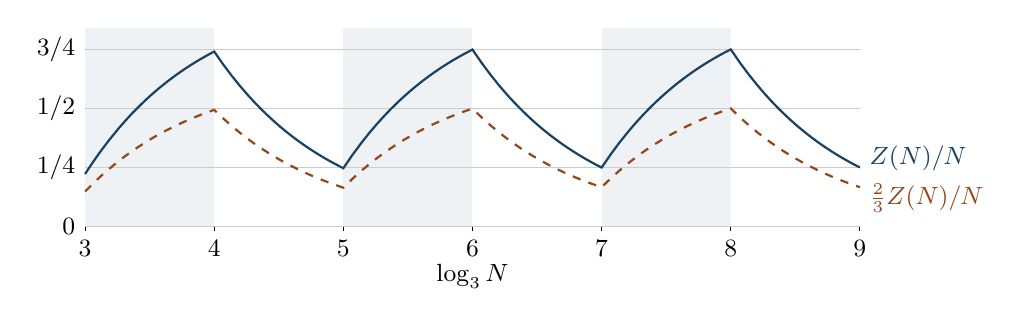
\begin{tikzpicture}[x=1.64cm,y=3.0cm,font=\small]
\fill[ink!7] (3,0) rectangle (4,.84);
\fill[ink!7] (5,0) rectangle (6,.84);
\fill[ink!7] (7,0) rectangle (8,.84);
\draw[black!20] (3,0) -- (9,0);
\node[left] at (3,0) {\(0\)};
\draw[black!20] (3,0.25) -- (9,0.25);
\node[left] at (3,0.25) {\(1/4\)};
\draw[black!20] (3,0.5) -- (9,0.5);
\node[left] at (3,0.5) {\(1/2\)};
\draw[black!20] (3,0.75) -- (9,0.75);
\node[left] at (3,0.75) {\(3/4\)};
\draw (3,0) -- ++(0,-.017) node[below] {\(3\)};
\draw (4,0) -- ++(0,-.017) node[below] {\(4\)};
\draw (5,0) -- ++(0,-.017) node[below] {\(5\)};
\draw (6,0) -- ++(0,-.017) node[below] {\(6\)};
\draw (7,0) -- ++(0,-.017) node[below] {\(7\)};
\draw (8,0) -- ++(0,-.017) node[below] {\(8\)};
\draw (9,0) -- ++(0,-.017) node[below] {\(9\)};
\node[below] at (6,-.12) {\(\log_3 N\)};
\draw[ink,thick] plot coordinates {
(3.000000,0.222222) (3.065045,0.275862) (3.125750,0.322581) (3.182658,0.363636) (3.261860,0.416667) (3.311074,0.447368) (3.357763,0.475000) (3.402174,0.500000)
(3.464974,0.533333) (3.504555,0.553191) (3.542487,0.571429) (3.578902,0.588235) (3.630930,0.611111) (3.664033,0.625000) (3.695975,0.637931) (3.726833,0.650000)
(3.771244,0.666667) (3.799691,0.676923) (3.827276,0.686567) (3.854050,0.695652) (3.892789,0.708333) (3.917729,0.716216) (3.942003,0.723684) (3.965647,0.730769)
(4.000000,0.740741) (4.065045,0.689655) (4.135485,0.638298) (4.200864,0.594059) (4.261860,0.555556) (4.311074,0.526316) (4.365317,0.495868) (4.416508,0.468750)
(4.464974,0.444444) (4.504555,0.425532) (4.548659,0.405405) (4.590723,0.387097) (4.630930,0.370370) (4.664033,0.357143) (4.701191,0.342857) (4.736891,0.329670)
(4.771244,0.317460) (4.799691,0.307692) (4.831793,0.297030) (4.862802,0.287081) (4.892789,0.277778) (4.917729,0.270270) (4.945987,0.262009) (4.973394,0.254237)
(5.000000,0.246914) (5.071993,0.304183) (5.138707,0.353357) (5.200864,0.396040) (5.261860,0.435185) (5.316381,0.468023) (5.367821,0.497253) (5.416508,0.523438)
(5.464974,0.548148) (5.508849,0.569412) (5.550706,0.588764) (5.590723,0.606452) (5.630930,0.623457) (5.667638,0.638340) (5.702923,0.652091) (5.736891,0.664835)
(5.771244,0.677249) (5.802798,0.688245) (5.833294,0.698517) (5.862802,0.708134) (5.892789,0.717593) (5.920458,0.726048) (5.947311,0.734012) (5.973394,0.741525)
(6.000000,0.748971) (6.071993,0.692015) (6.139779,0.642353) (6.202864,0.599341) (6.261860,0.561728) (6.316381,0.529070) (6.368654,0.499543) (6.418087,0.473137)
(6.464974,0.449383) (6.508849,0.428235) (6.551388,0.408683) (6.592027,0.390838) (6.630930,0.374486) (6.667638,0.359684) (6.703500,0.345788) (6.738002,0.332927)
(6.771244,0.320988) (6.802798,0.310051) (6.833794,0.299671) (6.863770,0.289963) (6.892789,0.280864) (6.920458,0.272455) (6.947752,0.264407) (6.974251,0.256820)
(7.000000,0.249657) (7.072762,0.307303) (7.140136,0.356723) (7.202864,0.399561) (7.261860,0.437243) (7.316969,0.470303) (7.368932,0.499695) (7.418087,0.525997)
(7.464974,0.549794) (7.509325,0.571205) (7.551615,0.590671) (7.592027,0.608447) (7.630930,0.624829) (7.668038,0.639816) (7.703692,0.653651) (7.738002,0.666463)
(7.771244,0.678424) (7.803142,0.689499) (7.833961,0.699835) (7.863770,0.709506) (7.892789,0.718621) (7.920761,0.727137) (7.947899,0.735152) (7.974251,0.742709)
(8.000000,0.749886) (8.072762,0.692275) (8.140255,0.642801) (8.203086,0.599927) (8.261860,0.562414) (8.316969,0.529374) (8.369024,0.499949) (8.418262,0.473623)
(8.464974,0.449931) (8.509325,0.428534) (8.551691,0.409046) (8.592172,0.391252) (8.630930,0.374943) (8.668038,0.359965) (8.703756,0.346113) (8.738125,0.333288)
(8.771244,0.321380) (8.803142,0.310312) (8.834016,0.299963) (8.863877,0.290283) (8.892789,0.281207) (8.920761,0.272697) (8.947948,0.264673) (8.974346,0.257107)
(9.000000,0.249962)
};
\draw[ochre,thick,dashed] plot coordinates {
(3.000000,0.148148) (3.065045,0.183908) (3.125750,0.215054) (3.182658,0.242424) (3.261860,0.277778) (3.311074,0.298246) (3.357763,0.316667) (3.402174,0.333333)
(3.464974,0.355556) (3.504555,0.368794) (3.542487,0.380952) (3.578902,0.392157) (3.630930,0.407407) (3.664033,0.416667) (3.695975,0.425287) (3.726833,0.433333)
(3.771244,0.444444) (3.799691,0.451282) (3.827276,0.457711) (3.854050,0.463768) (3.892789,0.472222) (3.917729,0.477477) (3.942003,0.482456) (3.965647,0.487179)
(4.000000,0.493827) (4.065045,0.459770) (4.135485,0.425532) (4.200864,0.396040) (4.261860,0.370370) (4.311074,0.350877) (4.365317,0.330579) (4.416508,0.312500)
(4.464974,0.296296) (4.504555,0.283688) (4.548659,0.270270) (4.590723,0.258065) (4.630930,0.246914) (4.664033,0.238095) (4.701191,0.228571) (4.736891,0.219780)
(4.771244,0.211640) (4.799691,0.205128) (4.831793,0.198020) (4.862802,0.191388) (4.892789,0.185185) (4.917729,0.180180) (4.945987,0.174672) (4.973394,0.169492)
(5.000000,0.164609) (5.071993,0.202788) (5.138707,0.235571) (5.200864,0.264026) (5.261860,0.290123) (5.316381,0.312016) (5.367821,0.331502) (5.416508,0.348958)
(5.464974,0.365432) (5.508849,0.379608) (5.550706,0.392509) (5.590723,0.404301) (5.630930,0.415638) (5.667638,0.425560) (5.702923,0.434728) (5.736891,0.443223)
(5.771244,0.451499) (5.802798,0.458830) (5.833294,0.465678) (5.862802,0.472089) (5.892789,0.478395) (5.920458,0.484032) (5.947311,0.489341) (5.973394,0.494350)
(6.000000,0.499314) (6.071993,0.461343) (6.139779,0.428235) (6.202864,0.399561) (6.261860,0.374486) (6.316381,0.352713) (6.368654,0.333028) (6.418087,0.315425)
(6.464974,0.299588) (6.508849,0.285490) (6.551388,0.272455) (6.592027,0.260558) (6.630930,0.249657) (6.667638,0.239789) (6.703500,0.230526) (6.738002,0.221951)
(6.771244,0.213992) (6.802798,0.206701) (6.833794,0.199780) (6.863770,0.193309) (6.892789,0.187243) (6.920458,0.181637) (6.947752,0.176271) (6.974251,0.171214)
(7.000000,0.166438) (7.072762,0.204868) (7.140136,0.237815) (7.202864,0.266374) (7.261860,0.291495) (7.316969,0.313536) (7.368932,0.333130) (7.418087,0.350664)
(7.464974,0.366529) (7.509325,0.380803) (7.551615,0.393781) (7.592027,0.405631) (7.630930,0.416552) (7.668038,0.426544) (7.703692,0.435768) (7.738002,0.444309)
(7.771244,0.452283) (7.803142,0.459666) (7.833961,0.466557) (7.863770,0.473004) (7.892789,0.479081) (7.920761,0.484758) (7.947899,0.490101) (7.974251,0.495140)
(8.000000,0.499924) (8.072762,0.461517) (8.140255,0.428534) (8.203086,0.399951) (8.261860,0.374943) (8.316969,0.352916) (8.369024,0.333299) (8.418262,0.315749)
(8.464974,0.299954) (8.509325,0.285689) (8.551691,0.272697) (8.592172,0.260835) (8.630930,0.249962) (8.668038,0.239977) (8.703756,0.230742) (8.738125,0.222192)
(8.771244,0.214253) (8.803142,0.206875) (8.834016,0.199976) (8.863877,0.193522) (8.892789,0.187471) (8.920761,0.181798) (8.947948,0.176448) (8.974346,0.171405)
(9.000000,0.166641)
};
\node[anchor=west,text=ink] at (9,.29) {\(Z(N)/N\)};
\node[anchor=west,text=ochre] at (9,.12) {\(\frac23 Z(N)/N\)};
\end{tikzpicture}

\caption{Exact finite counts for \(b=2,\ p=3\) and alternating phases \(1,0\). The curves join sampled values of the two main terms in Theorem~\ref{th:shell}. Shading marks zero shells. The peaks tend to \(3/4\) and \(1/2\).}\label{fig:prefix}
\end{figure}

For a binary word \(s=(s_0,s_1,\ldots)\), let \(\sigma s=(s_1,s_2,\ldots)\) and set
\[
 V_p(s)=(p-1)\sum_{i\ge0}\frac{s_i}{p^{i+1}} .
\]
Use lexicographic order with \(0<1\), and call \(s\) \emph{suffix-maximal} if \(\sigma^h s\le s\) for every \(h\ge1\).

\begin{theorem}[Attainable spectrum]\label{th:spectrum}
For each admissible \(b,p\), the set of values \(D_\infty(X)\) as the bounded integer phases vary is
\[
 \mathcal S_p=\{V_p(s):s\in\{0,1\}^{\mathbb N},\ \sigma^h s\le s\text{ for every }h\ge1\}.
\]
Every value has a realization with phases in \(\{0,1\}\). At \(p=2\), one suffix-maximal representation suffices at a dyadic endpoint.
\end{theorem}
\begin{proof}
By \eqref{eq:cycle}, \(H_j=V_p(h_j)\), where \(h_j=z_{j-1}z_{j-2}\cdots z_0 0^\infty\) and \(h_0=0^\infty\). The set \(K\) of subsequential limits of \(h_j\) is nonempty and compact in the product topology. Since \(\sigma h_j=h_{j-1}\) for \(j\ge1\), \(\sigma K\subseteq K\). Choose the largest allowable initial digit in \(K\), then the largest second digit with that prefix, and continue. The nested cylinders meet \(K\) in its lexicographically largest word \(s\). All suffixes of \(s\) belong to \(K\), hence are at most \(s\). Two words agreeing in \(k\) digits have values within \(p^{-k}\). At the first differing digit the gain from a 1 dominates the entire possible later loss, with a tie possible at \(p=2\). Thus \(V_p\) is continuous and nondecreasing. It follows that \(\limsup_j H_j=\max_{w\in K}V_p(w)=V_p(s)\).

Conversely, prescribe the chronological bits \(z_j\) by concatenating, for \(k=1,2,\ldots\), the blocks
\[
 0^k\,s_{k-1}s_{k-2}\cdots s_0 .
\]
During the padding the history value decreases. After \(1\le i\le k\) digits of the reversed prefix it starts with \(s_{k-i},\ldots,s_{k-1}\), followed by \(k\) zeros. The truncated value is at most \(V_p(\sigma^{k-i}s)\le V_p(s)\), and the contribution beyond the padding is at most \(p^{-(k+i)}\). At the end of the block the history agrees with \(s\) for \(k\) digits. The upper limit is therefore \(V_p(s)\). Taking \(c_j=1-z_j\) realizes the bits, with infinitely many nonzero phases even for the two constant words.
\end{proof}

\begin{corollary}\label{cor:symbol}
The spectrum is compact. Its smallest positive element is \(1-1/p\), and zero is its only isolated point. Periodic phase patterns are dense in the spectrum. For each suffix-maximal \(s\) and \(k\ge1\), one can use period \(2k\) to approximate \(V_p(s)\) within \(p^{-k}\).
\end{corollary}
\begin{proof}
The suffix inequalities are closed (a strict violation has a finite witness). Their set is compact and \(V_p\) continuous. Every nonzero admissible word begins with 1, and \(10^\infty\) attains the minimum. Repeating the padded block in the proof of Theorem~\ref{th:spectrum} gives the error bound: each block end agrees for \(k\) digits, and no intermediate history exceeds \(V_p(s)+p^{-k}\) in the limiting cycle.

Truncating an admissible word at any index and filling the rest with zeros preserves admissibility. In comparing a shifted truncation with the unshifted one, an earlier first difference retains its sign, and past the shifted cut the remaining digits on that side are zero. For a word with infinitely many ones, the truncations have strictly smaller values converging to its value. For a nonzero word with finite support, take \(k\) beyond its last one and repeat the padded block. At the block end the periodic history contains all its ones and further ones in the periodic tail. Its value is strictly greater while the error tends to zero.
\end{proof}

\begin{figure}[htbp]\centering
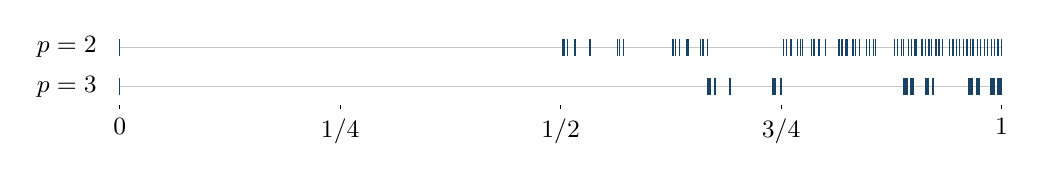
\begin{tikzpicture}[x=11.2cm,y=1cm,font=\small]
\draw[black!22] (0,0.95) -- (1,0.95);
\node[left] at (-.015,0.95) {\(p=2\)};
\draw[ink,line width=.5pt] (0.0000000,0.845) -- ++(0,.21);
\draw[ink,line width=.5pt] (0.5019608,0.845) -- ++(0,.21);
\draw[ink,line width=.5pt] (0.5039370,0.845) -- ++(0,.21);
\draw[ink,line width=.5pt] (0.5079365,0.845) -- ++(0,.21);
\draw[ink,line width=.5pt] (0.5161290,0.845) -- ++(0,.21);
\draw[ink,line width=.5pt] (0.5333333,0.845) -- ++(0,.21);
\draw[ink,line width=.5pt] (0.5647059,0.845) -- ++(0,.21);
\draw[ink,line width=.5pt] (0.5669291,0.845) -- ++(0,.21);
\draw[ink,line width=.5pt] (0.5714286,0.845) -- ++(0,.21);
\draw[ink,line width=.5pt] (0.6274510,0.845) -- ++(0,.21);
\draw[ink,line width=.5pt] (0.6299213,0.845) -- ++(0,.21);
\draw[ink,line width=.5pt] (0.6349206,0.845) -- ++(0,.21);
\draw[ink,line width=.5pt] (0.6431373,0.845) -- ++(0,.21);
\draw[ink,line width=.5pt] (0.6451613,0.845) -- ++(0,.21);
\draw[ink,line width=.5pt] (0.6588235,0.845) -- ++(0,.21);
\draw[ink,line width=.5pt] (0.6614173,0.845) -- ++(0,.21);
\draw[ink,line width=.5pt] (0.6666667,0.845) -- ++(0,.21);
\draw[ink,line width=.5pt] (0.7529412,0.845) -- ++(0,.21);
\draw[ink,line width=.5pt] (0.7559055,0.845) -- ++(0,.21);
\draw[ink,line width=.5pt] (0.7607843,0.845) -- ++(0,.21);
\draw[ink,line width=.5pt] (0.7619048,0.845) -- ++(0,.21);
\draw[ink,line width=.5pt] (0.7686275,0.845) -- ++(0,.21);
\draw[ink,line width=.5pt] (0.7716535,0.845) -- ++(0,.21);
\draw[ink,line width=.5pt] (0.7741935,0.845) -- ++(0,.21);
\draw[ink,line width=.5pt] (0.7843137,0.845) -- ++(0,.21);
\draw[ink,line width=.5pt] (0.7874016,0.845) -- ++(0,.21);
\draw[ink,line width=.5pt] (0.7921569,0.845) -- ++(0,.21);
\draw[ink,line width=.5pt] (0.7936508,0.845) -- ++(0,.21);
\draw[ink,line width=.5pt] (0.8000000,0.845) -- ++(0,.21);
\draw[ink,line width=.5pt] (0.8156863,0.845) -- ++(0,.21);
\draw[ink,line width=.5pt] (0.8188976,0.845) -- ++(0,.21);
\draw[ink,line width=.5pt] (0.8235294,0.845) -- ++(0,.21);
\draw[ink,line width=.5pt] (0.8253968,0.845) -- ++(0,.21);
\draw[ink,line width=.5pt] (0.8313725,0.845) -- ++(0,.21);
\draw[ink,line width=.5pt] (0.8346457,0.845) -- ++(0,.21);
\draw[ink,line width=.5pt] (0.8387097,0.845) -- ++(0,.21);
\draw[ink,line width=.5pt] (0.8470588,0.845) -- ++(0,.21);
\draw[ink,line width=.5pt] (0.8503937,0.845) -- ++(0,.21);
\draw[ink,line width=.5pt] (0.8549020,0.845) -- ++(0,.21);
\draw[ink,line width=.5pt] (0.8571429,0.845) -- ++(0,.21);
\draw[ink,line width=.5pt] (0.8784314,0.845) -- ++(0,.21);
\draw[ink,line width=.5pt] (0.8818898,0.845) -- ++(0,.21);
\draw[ink,line width=.5pt] (0.8862745,0.845) -- ++(0,.21);
\draw[ink,line width=.5pt] (0.8888889,0.845) -- ++(0,.21);
\draw[ink,line width=.5pt] (0.8941176,0.845) -- ++(0,.21);
\draw[ink,line width=.5pt] (0.8976378,0.845) -- ++(0,.21);
\draw[ink,line width=.5pt] (0.9019608,0.845) -- ++(0,.21);
\draw[ink,line width=.5pt] (0.9032258,0.845) -- ++(0,.21);
\draw[ink,line width=.5pt] (0.9098039,0.845) -- ++(0,.21);
\draw[ink,line width=.5pt] (0.9133858,0.845) -- ++(0,.21);
\draw[ink,line width=.5pt] (0.9176471,0.845) -- ++(0,.21);
\draw[ink,line width=.5pt] (0.9206349,0.845) -- ++(0,.21);
\draw[ink,line width=.5pt] (0.9254902,0.845) -- ++(0,.21);
\draw[ink,line width=.5pt] (0.9291339,0.845) -- ++(0,.21);
\draw[ink,line width=.5pt] (0.9333333,0.845) -- ++(0,.21);
\draw[ink,line width=.5pt] (0.9411765,0.845) -- ++(0,.21);
\draw[ink,line width=.5pt] (0.9448819,0.845) -- ++(0,.21);
\draw[ink,line width=.5pt] (0.9490196,0.845) -- ++(0,.21);
\draw[ink,line width=.5pt] (0.9523810,0.845) -- ++(0,.21);
\draw[ink,line width=.5pt] (0.9568627,0.845) -- ++(0,.21);
\draw[ink,line width=.5pt] (0.9606299,0.845) -- ++(0,.21);
\draw[ink,line width=.5pt] (0.9647059,0.845) -- ++(0,.21);
\draw[ink,line width=.5pt] (0.9677419,0.845) -- ++(0,.21);
\draw[ink,line width=.5pt] (0.9725490,0.845) -- ++(0,.21);
\draw[ink,line width=.5pt] (0.9763780,0.845) -- ++(0,.21);
\draw[ink,line width=.5pt] (0.9803922,0.845) -- ++(0,.21);
\draw[ink,line width=.5pt] (0.9841270,0.845) -- ++(0,.21);
\draw[ink,line width=.5pt] (0.9882353,0.845) -- ++(0,.21);
\draw[ink,line width=.5pt] (0.9921260,0.845) -- ++(0,.21);
\draw[ink,line width=.5pt] (0.9960784,0.845) -- ++(0,.21);
\draw[ink,line width=.5pt] (1.0000000,0.845) -- ++(0,.21);
\draw[black!22] (0,0.45) -- (1,0.45);
\node[left] at (-.015,0.45) {\(p=3\)};
\draw[ink,line width=.5pt] (0.0000000,0.345) -- ++(0,.21);
\draw[ink,line width=.5pt] (0.6667683,0.345) -- ++(0,.21);
\draw[ink,line width=.5pt] (0.6669716,0.345) -- ++(0,.21);
\draw[ink,line width=.5pt] (0.6675824,0.345) -- ++(0,.21);
\draw[ink,line width=.5pt] (0.6694215,0.345) -- ++(0,.21);
\draw[ink,line width=.5pt] (0.6750000,0.345) -- ++(0,.21);
\draw[ink,line width=.5pt] (0.6914634,0.345) -- ++(0,.21);
\draw[ink,line width=.5pt] (0.6916743,0.345) -- ++(0,.21);
\draw[ink,line width=.5pt] (0.6923077,0.345) -- ++(0,.21);
\draw[ink,line width=.5pt] (0.7408537,0.345) -- ++(0,.21);
\draw[ink,line width=.5pt] (0.7410796,0.345) -- ++(0,.21);
\draw[ink,line width=.5pt] (0.7417582,0.345) -- ++(0,.21);
\draw[ink,line width=.5pt] (0.7435976,0.345) -- ++(0,.21);
\draw[ink,line width=.5pt] (0.7438017,0.345) -- ++(0,.21);
\draw[ink,line width=.5pt] (0.7490854,0.345) -- ++(0,.21);
\draw[ink,line width=.5pt] (0.7493138,0.345) -- ++(0,.21);
\draw[ink,line width=.5pt] (0.7500000,0.345) -- ++(0,.21);
\draw[ink,line width=.5pt] (0.8890244,0.345) -- ++(0,.21);
\draw[ink,line width=.5pt] (0.8892955,0.345) -- ++(0,.21);
\draw[ink,line width=.5pt] (0.8899390,0.345) -- ++(0,.21);
\draw[ink,line width=.5pt] (0.8901099,0.345) -- ++(0,.21);
\draw[ink,line width=.5pt] (0.8917683,0.345) -- ++(0,.21);
\draw[ink,line width=.5pt] (0.8920403,0.345) -- ++(0,.21);
\draw[ink,line width=.5pt] (0.8925620,0.345) -- ++(0,.21);
\draw[ink,line width=.5pt] (0.8972561,0.345) -- ++(0,.21);
\draw[ink,line width=.5pt] (0.8975297,0.345) -- ++(0,.21);
\draw[ink,line width=.5pt] (0.8981707,0.345) -- ++(0,.21);
\draw[ink,line width=.5pt] (0.8983516,0.345) -- ++(0,.21);
\draw[ink,line width=.5pt] (0.9000000,0.345) -- ++(0,.21);
\draw[ink,line width=.5pt] (0.9137195,0.345) -- ++(0,.21);
\draw[ink,line width=.5pt] (0.9139982,0.345) -- ++(0,.21);
\draw[ink,line width=.5pt] (0.9146341,0.345) -- ++(0,.21);
\draw[ink,line width=.5pt] (0.9148352,0.345) -- ++(0,.21);
\draw[ink,line width=.5pt] (0.9164634,0.345) -- ++(0,.21);
\draw[ink,line width=.5pt] (0.9167429,0.345) -- ++(0,.21);
\draw[ink,line width=.5pt] (0.9173554,0.345) -- ++(0,.21);
\draw[ink,line width=.5pt] (0.9219512,0.345) -- ++(0,.21);
\draw[ink,line width=.5pt] (0.9222324,0.345) -- ++(0,.21);
\draw[ink,line width=.5pt] (0.9228659,0.345) -- ++(0,.21);
\draw[ink,line width=.5pt] (0.9230769,0.345) -- ++(0,.21);
\draw[ink,line width=.5pt] (0.9631098,0.345) -- ++(0,.21);
\draw[ink,line width=.5pt] (0.9634035,0.345) -- ++(0,.21);
\draw[ink,line width=.5pt] (0.9640244,0.345) -- ++(0,.21);
\draw[ink,line width=.5pt] (0.9642857,0.345) -- ++(0,.21);
\draw[ink,line width=.5pt] (0.9658537,0.345) -- ++(0,.21);
\draw[ink,line width=.5pt] (0.9661482,0.345) -- ++(0,.21);
\draw[ink,line width=.5pt] (0.9667683,0.345) -- ++(0,.21);
\draw[ink,line width=.5pt] (0.9669421,0.345) -- ++(0,.21);
\draw[ink,line width=.5pt] (0.9713415,0.345) -- ++(0,.21);
\draw[ink,line width=.5pt] (0.9716377,0.345) -- ++(0,.21);
\draw[ink,line width=.5pt] (0.9722561,0.345) -- ++(0,.21);
\draw[ink,line width=.5pt] (0.9725275,0.345) -- ++(0,.21);
\draw[ink,line width=.5pt] (0.9740854,0.345) -- ++(0,.21);
\draw[ink,line width=.5pt] (0.9743824,0.345) -- ++(0,.21);
\draw[ink,line width=.5pt] (0.9750000,0.345) -- ++(0,.21);
\draw[ink,line width=.5pt] (0.9878049,0.345) -- ++(0,.21);
\draw[ink,line width=.5pt] (0.9881061,0.345) -- ++(0,.21);
\draw[ink,line width=.5pt] (0.9887195,0.345) -- ++(0,.21);
\draw[ink,line width=.5pt] (0.9890110,0.345) -- ++(0,.21);
\draw[ink,line width=.5pt] (0.9905488,0.345) -- ++(0,.21);
\draw[ink,line width=.5pt] (0.9908509,0.345) -- ++(0,.21);
\draw[ink,line width=.5pt] (0.9914634,0.345) -- ++(0,.21);
\draw[ink,line width=.5pt] (0.9917355,0.345) -- ++(0,.21);
\draw[ink,line width=.5pt] (0.9960366,0.345) -- ++(0,.21);
\draw[ink,line width=.5pt] (0.9963403,0.345) -- ++(0,.21);
\draw[ink,line width=.5pt] (0.9969512,0.345) -- ++(0,.21);
\draw[ink,line width=.5pt] (0.9972527,0.345) -- ++(0,.21);
\draw[ink,line width=.5pt] (0.9987805,0.345) -- ++(0,.21);
\draw[ink,line width=.5pt] (0.9990851,0.345) -- ++(0,.21);
\draw[ink,line width=.5pt] (0.9996951,0.345) -- ++(0,.21);
\draw[ink,line width=.5pt] (1.0000000,0.345) -- ++(0,.21);
\draw (0,.22) -- ++(0,-.055) node[below] {\(0\)};
\draw (0.25,.22) -- ++(0,-.055) node[below] {\(1/4\)};
\draw (0.5,.22) -- ++(0,-.055) node[below] {\(1/2\)};
\draw (0.75,.22) -- ++(0,-.055) node[below] {\(3/4\)};
\draw (1,.22) -- ++(0,-.055) node[below] {\(1\)};
\end{tikzpicture}

\caption{Exact finite subset of \(\mathcal S_p\). Each tick is the largest cyclic history value of a binary period of length at most eight. Corollary~\ref{cor:symbol} gives \(1-1/p\) as the least positive value in the full spectrum; the ticks represent only the displayed finite periods.}\label{fig:spectrum}
\end{figure}

For binary lexicographic order these are the sup-words of Kaneko and Steiner \cite[Theorem~1 and \S4.1]{kanekosteiner}. They prove density of periodic sup-words and identify \(10^\infty\) as the least nonzero word. Theorem~\ref{th:spectrum} realizes the numerical image of this symbolic set as the upper discrepancies of the signed arithmetic family. Parry characterized admissible \(\beta\)-expansions \cite{parry}. Baiocchi and Komornik's Theorem~2.5(a) identifies the infinite expansions of one (infinitely many nonzero digits) that satisfy this suffix condition as the quasi-greedy expansions of one in varying bases \cite{bk}. Here \(V_p\) evaluates in one prescribed integer radix and includes terminating words. The two-sided univoque conditions also constrain the complemented word \cite{devries}; Allouche studies their self-Sturmian specialization \cite{allouche}.

For the doubling map, survivor sets and their bifurcations were studied by
Urba\'nski \cite{urbanski} and Nilsson \cite{nilsson}. At \(p=2\) the correspondence with the parameter set in Carminati and Tiozzo \cite[\S2]{ct} is explicit: \(1-\mathcal S_2\) consists of the parameters \(t\in[0,1]\) whose doubling orbit avoids \((0,t)\). Indeed complementing the digits gives a suffix-minimal expansion of \(t\). Except for \(t=0\) it has infinitely many ones: an admissible maximal word eventually all ones must be all ones. Use this nonterminating convention for \(t>0\); each suffix then represents the doubling iterate, taking value 1 at the circle point zero. Lexicographic and numerical comparisons agree on these expansions. Avoidance is exactly the assertion that every suffix is at least the original word. Complementing again gives the converse, including \(t=1\).


\section{Small positive discrepancies and transcendence}\label{sec:small}
The gap above zero in \(\mathcal S_p\) depends on keeping the translation fixed. By Theorem~\ref{th:shell} the spectrum for fixed \(m\ne0,r\in\Q\) is \(d_b(r)\mathcal S_p\). The factor is positive because a finite orbit leaves an interval of positive length empty. To make it small in any radix, one can prescribe a finite periodic orbit.

\begin{proposition}[De Bruijn translations]\label{th:bruijn}
Let \(w\) be a base-\(b\) cyclic de Bruijn word of order \(h\ge1\), \(L=b^h\), and \(A\) the base-\(b\) integer encoded by its \(L\) digits, including leading zeros. Put \(r=A/(b^L-1)\), and let \(y_0<\cdots<y_{L-1}\) be the points of its radix orbit. Then
\[
 d_b(r)=\frac{1+y_{L-1}-y_0}{L},\qquad
 \frac1L\le d_b(r)<\frac2L .
\]
Thus for each fixed signed expansion \(X\) with \(D_\infty(X)>0\), the translates obtained by taking successively higher orders have strictly positive upper discrepancies tending to zero.
\end{proposition}
\begin{proof}
The directed graph on words of length \(h-1\) has an edge for each length-\(h\) word, from its prefix to its suffix. Every vertex has \(b\) incoming and \(b\) outgoing edges, and successive appending of the letters of a target word reaches that vertex. An Euler circuit gives the required cyclic word, including the one-vertex case \(h=1\) \cite{debruijn,good}. The expansion of \(r\) repeats \(w\). Its rotations have distinct initial \(h\)-digit words, hence give one point in each cell \([j/L,(j+1)/L)\).

For \(L\) sorted distinct atoms of equal weight, the centered distribution function \(G(t)=\nu_r([0,t))-t\) has slope \(-1\) between atoms. At \(y_j\) its left value is \(j/L-y_j\) and its right limit is \((j+1)/L-y_j\). Since centered interval masses are increments of \(G\), the discrepancy is its oscillation on the circle, namely
\[
 \frac1L+\max_j(j/L-y_j)-\min_j(j/L-y_j).
\]
Write \(Ly_j=j+v_j\). The \(v_j=\fr{b^hy_j}\) permute the original points, because shifting by \(h\) permutes the cyclic rotations. Substitution gives the formula. The conclusion follows from Theorem~\ref{th:shell}.
\end{proof}

For \(b=2\) the word \(0011\) gives \(r=1/5\) and factor \(2/5\). The word \(00010111\) gives \(r=23/255\); the least and greatest rotations encode 23 and 226, giving factor \(229/1020\). For the alternating phases in Table~\ref{tab:cycles} the latter translate has upper discrepancy \(229/1360\). De Bruijn blocks also appear in constructions of infinite normal words and estimates for their discrepancy \cite{bcarton}. Here one finite cycle supplies the factor of a positive upper discrepancy.

There is a second choice in every radix. If \((b,t)=1\) and \(t\ge2\), then \(d_b(t^{-k})\to0\). Indeed, for \(q=t^k\) the proof of Lemma~\ref{lem:orbits} gives \(\ord_q(b)\gg q\). Apply the lemma to one full period and divide the \(o(q)\) count error by its length. For the same binary alternating example \(Y\), one obtains
\[
 D_\infty(Y+3^{-k})=\frac{1}{2\cdot3^{k-1}}\qquad(k\ge1).
\]
In fact \(\ord_{3^k}(2)=2\cdot3^{k-1}\), since an exponent giving 1 is even and \(v_3(4^u-1)=1+v_3(u)\). The orbit comprises all units modulo \(q=3^k\). For the \(L=2q/3\) sorted fractions with paired numerators \(3j+1,3j+2\), the offsets (index divided by \(L\), minus point) are \(-1/q,-1/(2q)\). The oscillation formula gives \(d_2(1/q)=2/q\).

The integer multiplier hypothesis matters even for one signed expansion. Altering \(c_0\) by one adds \(1/2-1/8=3/8\) when \(b=2,p=3\). Hence \(X'=9Y+3/8\) is a signed expansion whose zero pattern eventually agrees with that of \(Y\), giving \(D_\infty(X')=3/4\). But \(X'/9=Y+1/24\), and the eventual binary cycle of \(1/24\) is that of \(1/3\). Thus \(D_\infty(X'/9)=1/2\).

\begin{theorem}[Arithmetic nature of the realizations]\label{th:trans}
For bounded integer phases in \eqref{eq:X}, \(X\) is rational if the phases are eventually zero and transcendental otherwise. The conclusion holds for any integers \(b,p\ge2\), even when \(p\) is composite or divides \(b\). Under the hypotheses of Theorem~\ref{th:shell}, every element of \(\mathcal S_p\) has a transcendental realization. For each of the three phase periods in Table~\ref{tab:cycles}, \(mX+r\) is transcendental for every \(m\in\Z\setminus\{0\}\) and \(r\in\Q\).
\end{theorem}
\begin{proof}
The partial sum \(R_j\) has reduced denominator \(q_j\) dividing \(Q_j=p^j b^{p^j}\). For a bound \(C\ge1\) on the phases,
\[
 |X-R_j|\le\frac{2(p+1)C}{p^{j+1}b^{p^{j+1}}},
\]
by summing the geometric majorant over all integer radix exponents from \(p^{j+1}\) onwards. In particular \(Q_j|X-R_j|\to0\). If \(X=u/v\) is rational, \(v>0\), then every unequal partial sum has \(|X-R_j|\ge1/(vQ_j)\), so \(R_j=X\) eventually. Thus \(a_{j+1}=0\) eventually. The resulting relation \(c_{j+1}=pc_j\) and boundedness force the phases to be eventually zero. Conversely those phases give a finite rational sum.

Kano also uses lacunary partial sums and restricted denominators for transcendence \cite[Theorem~2]{kano}. For irrational \(X\), the \(R_j\) include infinitely many distinct reduced fractions. For fixed \(1<\mu<p\), the preceding tail bound implies \(0<|X-R_j|<Q_j^{-\mu}\le q_j^{-\mu}\) eventually, since \((p-\mu)p^j\log b\) dominates \(O(j)\). For \(p>2\), choose \(\mu>2\) and apply Roth's theorem \cite{roth}. For every \(p\ge2\), the prime divisors of \(q_j\) belong to the fixed finite set of prime divisors of \(pb\). For a reduced approximant \(u_j/q_j\), convergence to \(X\) gives \(|u_j|=O(q_j)\). Its height is therefore \(O(q_j)\). Ridout's restricted-denominator theorem excludes infinitely many such approximants with exponent \(\mu>1\) for an algebraic irrational \cite{ridout}. This proves transcendence. The padding in Theorem~\ref{th:spectrum} supplies infinitely many nonzero phases, as do the three periodic words. A rational affine map of nonzero slope preserves transcendence.
\end{proof}

\appendix
\section{An explicit pair of positive normal summands}\label{app:pair}
Here the summands are normal in the observation radix although their defining
series can use different dilations. They need not be the two standard
common-base generators of the Bailey--Borwein question.

\begin{theorem}\label{th:pair}
Suppose \(b\ge2\), \(c\ge3\) is odd, \(1\le m<\ell<c\), and \(c\mid b^{\ell-m}+1\). Then \(x=mT_{b,c,m}\) and \(y=\ell T_{b,c,\ell}\) are positive and normal in base \(b\). Their sum is irrational and nonnormal. For every \(h\ge1\),
\[
 \limsup_{N\to\infty}\mu_{N,x+y}([0,b^{-h}))\ \ge\ \frac{c-\ell}{c-1}.
\]
For every \(b\ge2\) and every real \(\eta<1\), one explicit choice of \(c,m,\ell\) makes this lower bound exceed \(\eta\), simultaneously for all \(h\).
\end{theorem}
\begin{proof}
The divisibility implies \((b,c)=1\). For any fixed \(m\ge1\), on \([mc^j,mc^{j+1})\) the completed part of the shifted \(mT_{b,c,m}\) follows a radix orbit of denominator \(q=c^j\). At the left endpoint its numerator with denominator \(q\) is \(1\bmod c\) for \(j\ge1\), since all previous insertions have a factor \(c\) after clearing. The omitted positive tail is at most \(\sum_{i>j}c^{-i}=1/((c-1)c^j)\) throughout the shell. By Lemma~\ref{lem:orbits} on the fixed prime support of \(c\), every partial shell has centered interval counts \(o(c^j)\) for the completed orbit. Summing and applying Lemma~\ref{lem:perturb} proves normality of the real series. Positivity follows from its terms.

Set \(B=b^{\ell-m}\). For each \(j\ge0\), \(c^{j+1}\mid B^{c^j}+1\). Indeed, for \(v\equiv-1\bmod c\) the quotient \((v^c+1)/(v+1)\) is divisible by \(c\), since its alternating sum has \(c\) terms all congruent to 1 modulo \(c\). Induction from \(c\mid B+1\) proves the claim. On \([\ell c^k,c^{k+1})\), every completed pair indexed by \(j\le k\) therefore contributes the integer
\[
 b^{n-\ell c^j}\frac{1+B^{c^j}}{c^j}.
\]
The remaining shifted tail lies in \((0,2/((c-1)c^k)]\). A rational of denominator \(v\) has all its shifted fractional parts on the grid \(v^{-1}\Z\), so these strictly positive, arbitrarily small remainders imply irrationality. For fixed \(h\), all sufficiently late positions in these intervals give \(h\) zero digits. At \(N=c^{k+1}\) their lengths from scales \(j_0\) through \(k\) sum to \((c-\ell)\sum_{j=j_0}^k c^j\). Division by \(N\) gives the asserted lower bound. For large \(h\) it exceeds the normal frequency \(b^{-h}\).

Take \(m=1,\ \ell=2d+1\) and \(c\) the odd part of \(b^{2d}+1\). For even \(b\) the number \(b^{2d}+1\) is odd, and for odd \(b\) it is \(2\bmod 4\). Therefore \(c\ge(b^{2d}+1)/2\), and \(1-2d/(c-1)\to1\) as \(d\to\infty\). Any sufficiently large \(d\) works.
\end{proof}

\section*{Formal verification and reproducibility}
The arithmetic statements cited below refer to the Lean sources at
\href{https://github.com/eldernos/MathematicsResearch/tree/a09e011720bc74396a27f4cb3ce2d8a5b3ce5035}{Checkpoint 11, revision \texttt{a09e011720bc}}.
The companion \texttt{CORRESPONDENCE.md} records the full declaration names, hypotheses and evidence for each numbered result.
\begin{center}\small
\begin{tabular}{@{}ll@{}}
\toprule
Result & Pinned formal statement\\
\midrule
Theorem~\ref{th:cyclo} (CR-01) & \source{CyclotomicClassification}{99}{Cyclotomic equivalence}, \source{CyclotomicDistribution}{74}{endpoint distribution}\\
Theorem~\ref{th:shell} (DS-01, DS-03) & \source{SignedShellDiscrepancy}{144}{Untranslated prefixes}, \source{TranslatedShells}{198}{translated prefixes}, \source{TranslatedShells}{221}{product}\\
Proposition~\ref{th:periodic} (DS-02) & \source{SignedShellDiscrepancy}{335}{Periodic maximum}, \source{SignedShellDiscrepancy}{411}{three evaluations}\\
Theorem~\ref{th:spectrum} (DS-04) & \source{ShellHistories}{388}{Attainable discrepancy equivalence}\\
Proposition~\ref{th:bruijn} & \source{TranslatedShellExamples}{50}{Positivity and upper bound from cell counts}, \source{TranslatedShellExamples}{82}{eight-cell example}\\
Theorem~\ref{th:trans} & \source{SignedShellDiscrepancy}{448}{Irrationality under prime and coprimality hypotheses}\\
Theorem~\ref{th:pair} & \source{StonehamComponents}{138}{Every-radix pair of normal summands}\\
\bottomrule
\end{tabular}
\end{center}
The rational de Bruijn equality, \eqref{eq:finitebridge}, the composite-parameter extension of the irrationality criterion, and the transcendence conclusions have the paper proofs above. Roth and Ridout are external inputs. From the manuscript directory, run \texttt{python3 figures/generate.py} and \texttt{latexmk -pdf paper.tex}. The figure data, Lean correspondence checks and literature search record accompany the source.

\paragraph{AI assistance.} OpenAI Codex drafted the exposition, compared it with the cited declarations and prepared the figures.

\bibliographystyle{plain}
\begingroup
\let\originalbibliography\thebibliography
\renewcommand{\thebibliography}[1]{\originalbibliography{#1}\small\setlength{\itemsep}{2pt}}
\bibliography{references}
\endgroup
\end{document}
